If the program window can be displayed normally, you can enter the value for verification. The conditions of 1, 2, 3 and 4, 5 and 6, 7 in the project requirement file are similar, so we choose 1(Figure.\ref{fig:eg1}), 4(Figure.\ref{fig:eg4}), and 6(Figure.\ref{fig:eg6}) as the demo of our program.
\begin{figure}[!htbp]
	\centering
	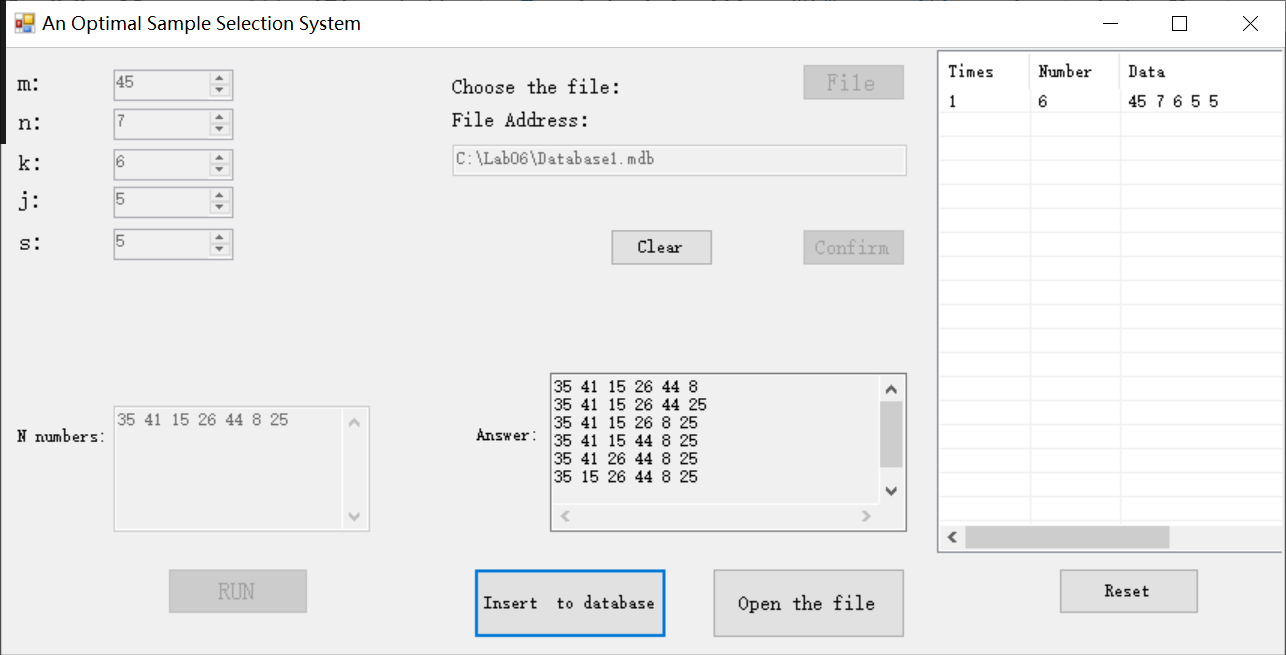
\includegraphics[width=0.75\textwidth]{images/1.png}
	\caption{E.g.$1$: Input the data: $m=45, n=7, k=6, j=5, s=5.$}
	\label{fig:eg1}
\end{figure}
\begin{figure}[!htbp]
	\centering
	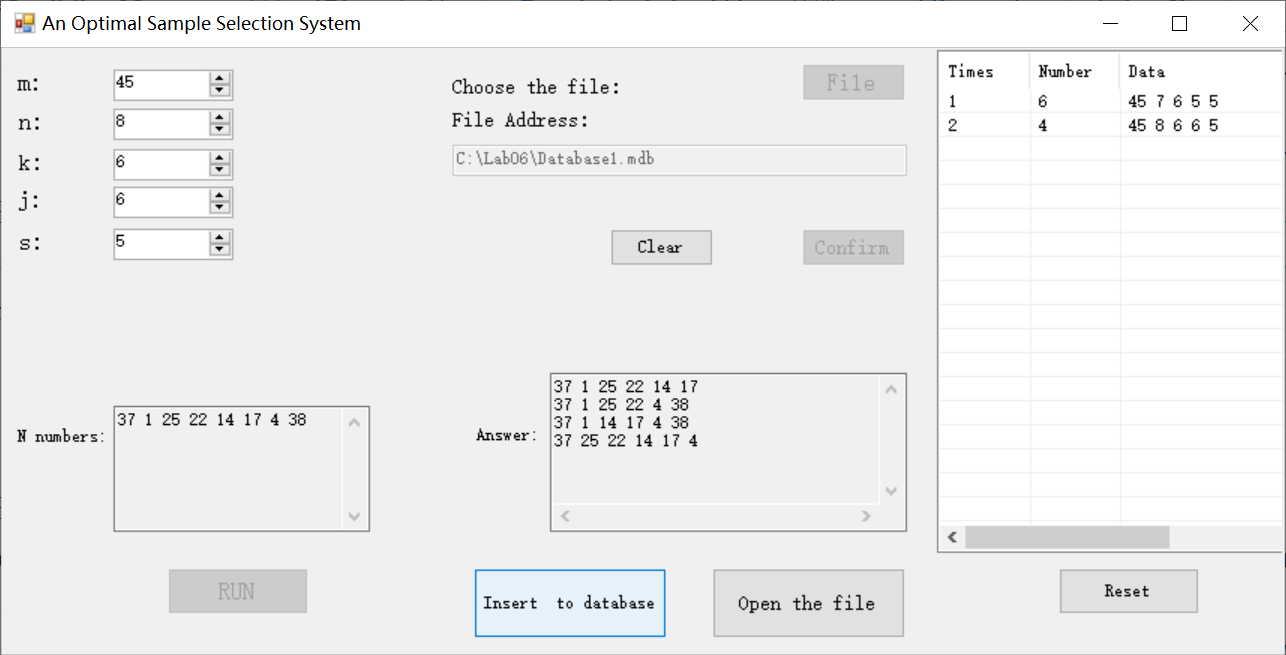
\includegraphics[width=0.75\textwidth]{images/4.png}
	\caption{E.g.$4$: Input the data: $m=45, n=8, k=6, j=6, s=5.$}
	\label{fig:eg4}
\end{figure}
\begin{figure}[!htbp]
	\centering
	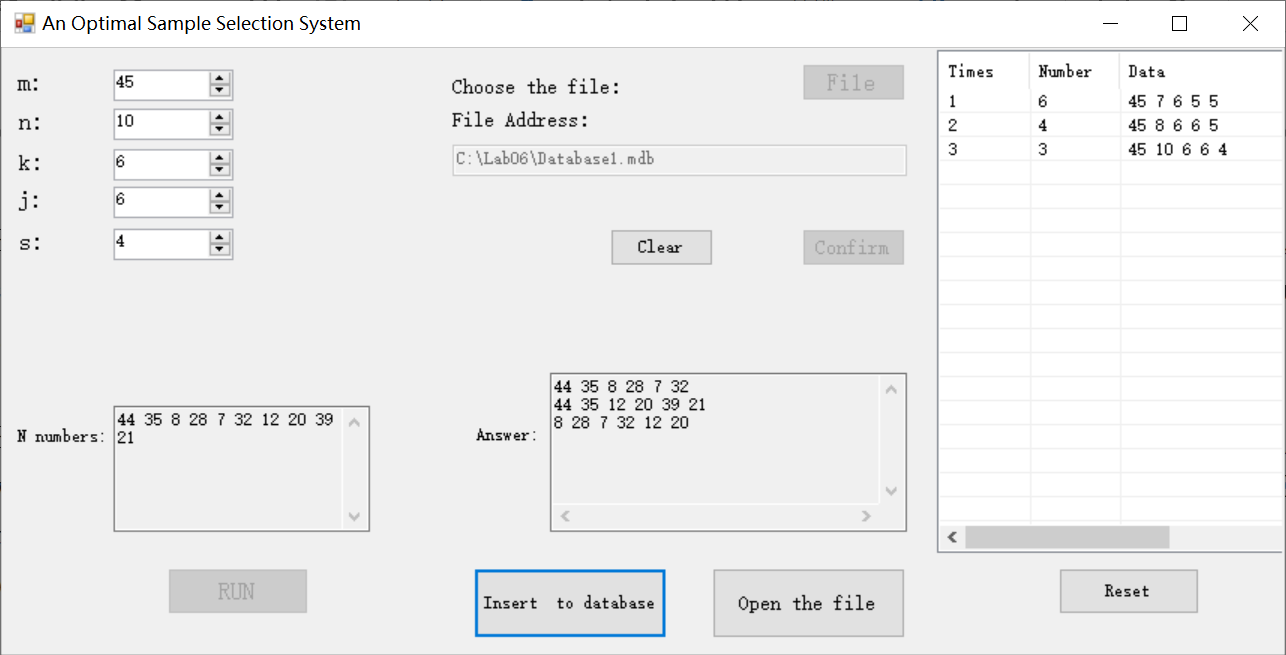
\includegraphics[width=0.75\textwidth]{images/6.png}
	\caption{E.g.$6$: Input the data: $m=45, n=10, k=6, j=6, s=4.$}
	\label{fig:eg6}
\end{figure}
% \begin{itemize}
% \item E.g.$1$: Input the data: $m=45, n=7, k=6, j=5, s=5.$
% \begin{center}
%     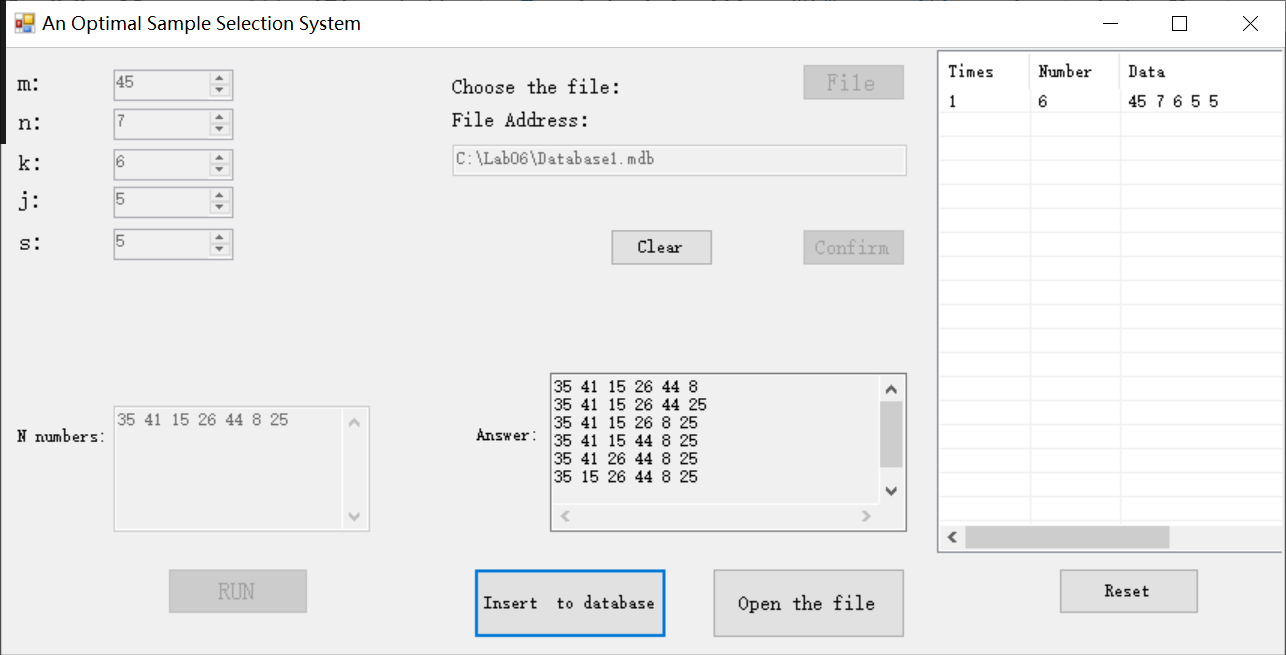
\includegraphics[width=10cm,height=6cm]{images/1.png}
% \end{center}

% \item E.g.$4$: Input the data: $m=45, n=8, k=6, j=6, s=5.$
% \begin{center}
%     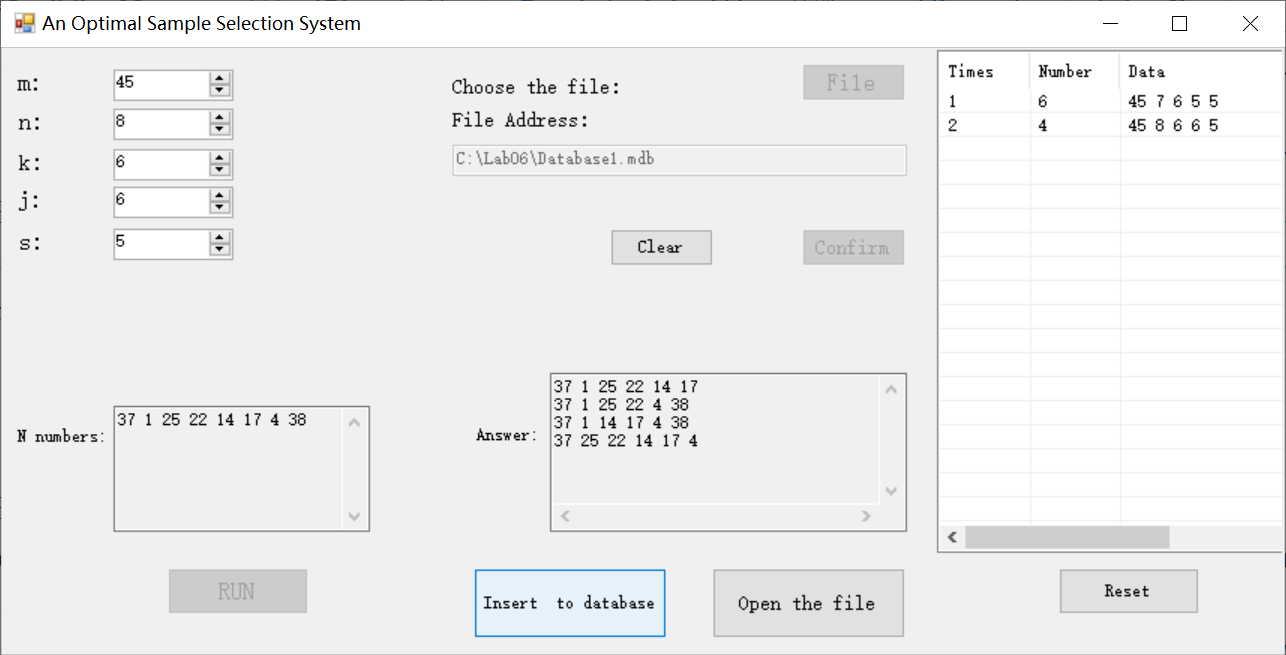
\includegraphics[width=10cm,height=6cm]{images/4.png}
% \end{center}

% \item E.g.$6$: Input the data: $m=45, n=10, k=6, j=6, s=4.$
% \begin{center}
%     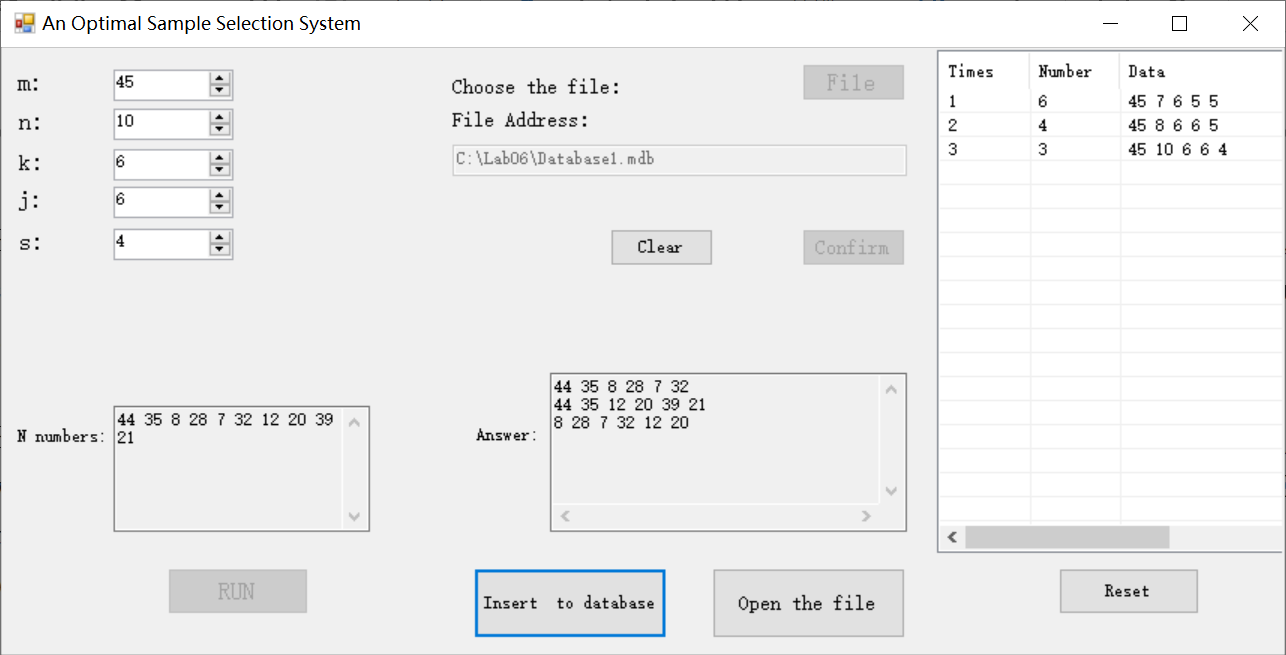
\includegraphics[width=10cm,height=6cm]{images/6.png}
% \end{center}

% \end{itemize}

